\documentclass[a4paper,11pt,oneside]{book}
\usepackage{setspace}
\usepackage{titling}
\usepackage{graphicx}
\usepackage{lipsum}
\usepackage{tabularx}  % Add in the preamble if not already
\usepackage{tocloft}   % For spacing if needed
\pagenumbering{roman}

\begin{document}

% ----------------- Title Page -----------------
\begin{titlepage}
    \centering
    \vspace*{2cm}
    {\Large\bfseries\uppercase{Use of Explainable AI using SHAP on Crop Yield Prediction in India} \par}
    \vspace{1cm}
    {\large Submitted in partial fulfilment of the requirements of the degree of\\[0.3cm]
    \textbf{Master of Technology} \par}
    \vspace{2.5cm}
    
    {\large by \par}
    \vspace{0.5cm}
    {\LARGE \textbf{Udit Jain} \par}
    {\Large (Roll No: 24CSM1R23) \par}
    \vspace{2.5cm}
    
    {\large Supervisor:\par}
    \vspace{0.3cm}
    \textbf{Dr. Manjubala Bisi} \\
    \textit{Assistant Professor, Department of CSE} \\[0.5cm]
    
    \vfill
    {\large Department of Computer Science and Engineering\\
    National Institute of Technology, Warangal\\
    India\\}
    \vspace{0.5cm}
    
    {\large \textbf{April 15, 2025} \par}
\end{titlepage}

% ----------------- Acknowledgement -----------------
\chapter*{Acknowledgement}
\addcontentsline{toc}{chapter}{Acknowledgement}
\vspace{1em}
I would like to express my sincere gratitude to my project supervisor, \textbf{Professor Manjubala Bisi}, Department of Computer Science and Engineering, National Institute of Technology Warangal, for her valuable guidance, encouragement, and continuous support throughout the course of this project. His/her insights, suggestions, and constructive feedback have been instrumental in shaping this work.

I also extend my heartfelt thanks to all the faculty members and staff of the Department of Computer Science and Engineering, NIT Warangal, for providing an excellent academic and research environment and for facilitating the resources required for successful completion of this project.

I would like to acknowledge the support of my friends and batchmates who contributed their ideas, encouragement, and assistance during the different phases of this work. Their moral support played a key role in keeping me motivated.

A special note of appreciation to my family for their unconditional support and constant encouragement throughout my academic journey.

Finally, I am grateful to the National Institute of Technology Warangal for providing the infrastructure and learning environment that enabled me to carry out this project successfully.

\vspace{1cm}

\begin{flushright}
\textbf{Udit Jain} \\
Roll No: 24CSM1R23
\end{flushright}

\newpage

% ----------------- Declaration -----------------
\chapter*{Declaration}
\addcontentsline{toc}{chapter}{Declaration}
\vspace{1em}
I declare that this written submission represents my ideas, and those of my supervisor, in my own words. Where others’ ideas or words have been included, I have adequately cited and referenced the original sources. I also declare that I have adhered to all principles of academic honesty and integrity and have not misrepresented, fabricated, or falsified any idea, data, fact, or source in this submission.

I understand that any violation of the above will be cause for disciplinary action by the Institute and can also evoke penal action from the original sources which have not been properly cited or acknowledged.

\vspace{2cm}
\begin{flushright}
(Signature) \\
\textbf{Udit Jain} \\
Roll No: 24CSM1R23
\end{flushright}

\newpage

% ----------------- Approval Sheet (Page 4) -----------------
% \chapter*{Approval Sheet}
% \addcontentsline{toc}{chapter}{Approval Sheet}

\begin{center}
    {\Huge \textbf{Approval Sheet}}
\end{center}
\vspace{1em}

\begin{center}
\vspace{1em}
This Dissertation Work entitled \\[0.5cm]
\textbf{"Use of Explainable AI using SHAP on Crop Yield Prediction in India"} \\[0.5cm]
by \textbf{Udit Jain (Roll No: 24CSM1R23)} \\[0.5cm]
is approved for the degree of \textbf{Master of Technology}.
\end{center}

\vspace{1cm}

\begin{center}
\textbf{Examiners:} \\ [0.5cm]
Dr. Manjubala Bisi , Dr. P Venkata Subba Reddy , Dr. Nidhi Sonkar \\
% \rule{10cm}{0.4pt} \\
\end{center}

\vspace{0.5cm}

\begin{center}
\textbf{Supervisor:} \\[0.5cm]
Dr. Manjubala Bisi \\
% \rule{10cm}{0.4pt} \\
\end{center}

\vspace{0.5cm}

\begin{center}
\textbf{Chairman:} \\[0.5cm]
Dr. Krishna M. Ella \\
% \rule{10cm}{0.4pt} \\
\end{center}

\vspace{0.5cm}

\begin{center}
\textbf{CSE (HOD):} \\[0.5cm]
Dr. R Padmavathy \\
% \rule{10cm}{0.4pt} \\
\end{center}

\vspace{0.5cm}

\begin{center}
National Institute of Technology, Warangal
\end{center}


\newpage

% ----------------- Certificate -----------------
\chapter*{Certificate}
\addcontentsline{toc}{chapter}{Certificate}
\vspace{1em}
This is to certify that the Dissertation work entitled \textbf{"Use of Explainable AI using SHAP on Crop Yield Prediction in India"} is a bonafide record of work carried out by \textbf{Udit Jain (Roll No: 24CSM1R23)}, submitted to the Department of Computer Science and Engineering, in partial fulfilment of the requirements for the award of the degree of \textbf{Master of Technology} at the \textbf{National Institute of Technology, Warangal} during the academic year 2024--2025.

\vspace{2cm}
\begin{flushleft}
(Signature) \\
\textbf{Dr. Manjubala Bisi} \\
Assistant Professor \\
Department of Computer Science and Engineering
\end{flushleft}

% \vspace{2cm}
% \begin{flushleft}
% (Signature) \\
% \textbf{Dr. Co-Supervisor Name} \\
% Designation \\
% Department of Computer Science and Engineering
% \end{flushleft}

\newpage

% ----------------- Abstract -----------------
\chapter*{\begin{center}\Huge Abstract\end{center}}
\addcontentsline{toc}{chapter}{Abstract}
\vspace{1em}
Accurate crop yield prediction is essential for resource optimization and food security, yet it remains a challenging task due to environmental variability and complex factors influencing agriculture. This project develops a crop yield prediction system that uses machine learning (ML) models such as Random Forest, XGBoost, and Decision Tree, with an emphasis on explainability through SHAP (SHapley Additive exPlanations).

SHAP, based on cooperative game theory, provides transparent insights into how features contribute to model predictions, making the models more interpretable for stakeholders like farmers and policymakers. The system is trained on agricultural data, and its performance is evaluated using metrics like accuracy, MAE, and RMSE. SHAP visualizations, including summary and force plots, help elucidate feature importance and individual prediction explanations.

The results show that Random Forest, integrated with SHAP, offers superior prediction accuracy and interpretability. This approach highlights the potential of explainable AI in agriculture, enabling data-driven decisions and enhancing trust in AI models.

\vspace{1cm}
\noindent\textbf{Keywords:} Explainable AI, SHAP, Crop Yield Prediction, Random Forest, XGBoost, Machine Learning

\newpage

% ----------------- Table of Contents (Custom Manual Entry) -----------------

\chapter*{Contents}
\addcontentsline{toc}{chapter}{Contents}

\begin{flushleft}
\begin{tabularx}{\textwidth}{@{}lXr@{}}
\textbf{Acknowledgement} & & ii \\
\textbf{Declaration} & & iii \\
\textbf{Certificate} & & iv \\
\textbf{Abstract} & & v \\
\\
\textbf{1 Introduction} & & 1 \\
\hspace{1em}1.1 Context and Motivation & & 1 \\
% \hspace{1em}1.2 Challenges in Current Systems & & 2 \\
\hspace{1em}1.2 Challenges in Current Systems & & 1 \\
\hspace{1em}1.3 Role of SHAP in Bridging the Gap & & 2 \\
\hspace{1em}1.4 Need for Explainability in Agriculture & & 2 \\
\hspace{1em}1.5 Objectives and Scope of the Project & & 2 \\
\hspace{1em}1.6 Expected Contributions & & 3 \\
\hspace{1em}1.7 Organization of the Report & & 3 \\
\\
\textbf{2 Background} & & 5 \\
\hspace{1em}2.1 Artificial Intelligence in Agriculture & & 5 \\
\hspace{1em}2.2 Crop Yield Prediction & & 6 \\
\hspace{1em}2.3 Machine Learning for Yield Prediction & & 6 \\
\hspace{1em}2.4 Explainable Artificial Intelligence (XAI) & & 7 \\
\hspace{1em}2.5 SHAP: SHapley Additive exPlanations & & 7 \\
\hspace{1em}2.6 Why SHAP for Crop Yield Prediction? & & 8 \\
\hspace{1em}2.7 Summary & & 8 \\
\end{tabularx}
\end{flushleft}

\newpage  % Force a page break here

\begin{flushleft}
\begin{tabularx}{\textwidth}{@{}lXr@{}}
\textbf{3 Related Work} & & 9 \\
\hspace{1em}3.1 AI-Based Approaches for Crop Yield Prediction & & 9 \\
\hspace{1em}3.2 Explainable AI in Agriculture & & 10 \\
\hspace{1em}3.3 Gaps in Current Research & & 11 \\
\hspace{1em}3.4 Need for This Study & & 11 \\
\hspace{1em}3.5 Summary & & 11 \\
\\
\textbf{4 Proposed Solution} & & 12 \\
\hspace{1em}4.1 System Overview & & 12 \\
\hspace{1em}4.2 Data Preprocessing & & 12 \\
\hspace{1em}4.3 Model Development and Training & & 13 \\
% \hspace{1em}4.4 SHAP Integration for Interpretability & & 19 \\
\hspace{1em}4.4 Model Evaluation Metrics & & 13 \\
\hspace{1em}4.5 SHAP: Mathematical Formulation & & 14 \\
\hspace{1em}4.6 SHAP-Based Interpretation & & 14 \\
\hspace{1em}4.7 Key Features Identified via SHAP From & & 15 \\
\hspace{1em}4.8 Workflow Summary & & 15 \\
\hspace{1em}4.9 Summary & & 16 \\
\\
\textbf{5 Experiments} & & 17 \\
\hspace{1em}5.1 Experimental Setup & & 17 \\
\hspace{1em}5.2 Model Evaluation Metrics & & 18 \\
\hspace{1em}5.3 Performance Comparison & & 18 \\
\hspace{1em}5.4 SHAP-Based Interpretability Results & & 18 \\
\hspace{1em}5.5 Interpretation of Results & & 18 \\
\hspace{1em}5.6 Comparison with Traditional Models & & 20 \\
\hspace{1em}5.7 Summary & & 21 \\
\\
\textbf{6 Conclusion and Future Work} & & 22 \\
\hspace{1em}6.1 Conclusion & & 22 \\
\hspace{1em}6.2 Implications of Findings & & 23 \\
\hspace{1em}6.3 Limitations & & 23 \\
\hspace{1em}6.4 Future Work & & 23 \\
\hspace{1em}6.5 Final Remarks & & 24 \\
\\
\textbf{References} & & 25 \\
\end{tabularx}
\end{flushleft}

\newpage

% ----------------- List of Figures -----------------

\chapter*{List of Figures}
\addcontentsline{toc}{chapter}{List of Figures} % Add to Table of Contents
\vspace{1em}

\listoffigures

\newpage

\pagenumbering{arabic}
% ----------------- Introduction -----------------


\chapter{Introduction}

India's economy is significantly driven by agriculture, a sector that sustains more than half of its population and ensures national food security. Predicting agricultural output, especially crop yield, is not only vital for individual farmers but also for policymakers, supply chain managers, and economists. With rising climate uncertainties, evolving cultivation practices, and increased demand for efficient food production systems, it is imperative to leverage technological innovations such as Artificial Intelligence (AI) to enhance agricultural forecasting.

\section{Context and Motivation}

In recent years, Machine Learning (ML) and Deep Learning (DL) algorithms have shown promising results in yield prediction. However, these models often act as “black boxes” — offering no insight into how predictions are made. This opacity reduces the trustworthiness of the system for stakeholders such as farmers and government officials, who need actionable insights, not just outputs. The inability to understand the decision-making process limits adoption and may lead to resistance against AI-based agricultural technologies.

To address this, Explainable AI (XAI) is introduced. XAI aims to make model behavior interpretable without sacrificing performance. SHAP (SHapley Additive exPlanations), one of the most robust XAI techniques, attributes the prediction output to each input feature based on principles from cooperative game theory. This makes AI-driven decisions more transparent, interpretable, and hence, trustworthy.

\section{Challenges in Current Systems}

Despite the growth in AI applications, several persistent challenges remain in crop yield prediction:

\begin{itemize}
    \item \textbf{Lack of Interpretability:} Most high-performing models fail to provide explanations for their predictions, making them untrustworthy for end-users.
    \item \textbf{Data Quality and Diversity:} Agricultural datasets are often noisy, sparse, and vary significantly across regions and seasons.
    \item \textbf{Variability in Environmental Conditions:} Changing climatic parameters such as rainfall, temperature, and soil conditions introduce complexity in accurate yield forecasting.
    \item \textbf{Inaccessibility for Farmers:} The technological gap between model creators and rural users can hinder the effective implementation of AI solutions.
\end{itemize}

\section{Role of SHAP in Bridging the Gap}

SHAP provides a unifying framework to quantify feature importance for individual predictions. It decomposes a model’s prediction into additive contributions from each input feature, giving users the ability to understand both global and local model behavior. This transparency can help:

\begin{itemize}
    \item Build trust in AI outputs.
    \item Identify critical yield-influencing factors (e.g., season, crop type, region).
    \item Provide personalized explanations for region-specific agricultural recommendations.
\end{itemize}

\section{Need for Explainability in Agriculture}

In a domain like agriculture where ground-level implementation is deeply affected by predictive insights, stakeholders demand transparency. Farmers, agronomists, and policy planners often make high-stakes decisions based on these outputs. Therefore, merely providing a prediction is insufficient — stakeholders must also understand why a certain crop is likely to yield more or less in a particular region or season.

\section{Objectives and Scope of the Project}

This project aims to bridge the gap between high-performance predictive modeling and human interpretability by integrating SHAP into a crop yield prediction pipeline. The scope of this project includes:

\begin{itemize}
    \item Gathering and preprocessing crop-related data from Indian states and districts.
    \item Training ML and DL models such as Random Forest, XGBoost, Decision Tree, and LSTM.
    \item Evaluating models using performance metrics like Accuracy, MAE, RMSE, and SD.
    \item Applying SHAP to the best-performing model (Random Forest) to explain predictions.
    \item Visualizing the impact of features using summary, waterfall, and decision plots.
\end{itemize}

\section{Expected Contributions}

The major contributions of this project are as follows:

\begin{itemize}
    \item A pipeline for interpretable crop yield prediction using real Indian agricultural datasets.
    \item Comparative evaluation of classical and deep learning models based on performance and explainability.
    \item Integration of SHAP to derive actionable insights for stakeholders.
    \item Visual analysis tools for model interpretation to support informed decision-making.
\end{itemize}

\section{Organization of the Report}

This report is structured as follows:

\begin{itemize}
    \item \textbf{Chapter 1: Introduction} — Provides background, motivation, challenges, and scope.
    \item \textbf{Chapter 2: Background} — Discusses foundational concepts of ML, DL, and XAI.
    \item \textbf{Chapter 3: Literature Survey} — Reviews existing models and gaps in crop yield prediction.
    \item \textbf{Chapter 4: Proposed Methodology} — Details the model development and SHAP integration process.
    \item \textbf{Chapter 5: Experimental Results} — Presents evaluation metrics, SHAP visualizations, and analysis.
    \item \textbf{Chapter 6: Conclusion and Future Work} — Summarizes findings and outlines future directions.
\end{itemize}


\newpage

% ----------------- Background -----------------


\chapter{Background}

Technological innovations such as Artificial Intelligence (AI) and Machine Learning (ML) have been instrumental in revolutionizing modern agriculture. From yield prediction and soil monitoring to pest detection and resource optimization, AI is playing an increasingly vital role in enhancing productivity and sustainability. However, the real value of these models is realized only when they are both accurate and interpretable—especially in agriculture, where decisions based on AI predictions have real-world implications for food security, economic planning, and farmer livelihoods.

\section{Artificial Intelligence in Agriculture}

AI refers to systems that mimic human intelligence to perform tasks such as learning, problem-solving, and pattern recognition. In agriculture, AI is used for:
\begin{itemize}
    \item Predicting crop yields based on historical and environmental data.
    \item Recommending optimal sowing and harvesting periods.
    \item Monitoring soil health and moisture levels using sensors and computer vision.
    \item Detecting plant diseases through image-based classification.
    \item Forecasting weather and irrigation needs.
\end{itemize}

By combining AI with large datasets collected from diverse regions and seasons, predictive models can generate insights that were previously difficult or impossible to obtain using traditional statistical methods.

\section{Crop Yield Prediction}

Crop yield prediction is one of the most critical tasks in precision agriculture. It involves forecasting the quantity of produce (yield) expected from a given crop in a specific area and time period. Accurate predictions help:
\begin{itemize}
    \item Enable farmers to plan resources more efficiently (water, fertilizer, labor).
    \item Assist policymakers in making decisions regarding food procurement and supply chains.
    \item Strengthen national food security by identifying possible shortages in advance.
\end{itemize}

The complexity of crop yield prediction arises from the multitude of influencing factors, including weather conditions, soil quality, crop variety, seasonality, and farming practices. ML and DL models can capture non-linear patterns and dependencies within these variables to improve prediction accuracy.

\section{Machine Learning for Yield Prediction}

ML models learn from past data to make future predictions. In agriculture, popular models include:

\begin{itemize}
    \item \textbf{Decision Tree (DT):} A flowchart-like structure where internal nodes represent decision rules and leaf nodes represent outcomes.
    \item \textbf{Random Forest (RF):} An ensemble of decision trees that improves prediction accuracy and reduces overfitting.
    \item \textbf{XGBoost:} An efficient boosting algorithm that builds trees sequentially, minimizing error at each step.
    \item \textbf{Recurrent Neural Networks (RNN) and LSTM:} Deep learning models suitable for sequential or time-series data, capturing long-term dependencies in crop patterns.
\end{itemize}

While these models perform well on metrics like accuracy and RMSE, they often lack the transparency required for real-world deployment. This limitation has sparked growing interest in Explainable AI (XAI).

\section{Explainable Artificial Intelligence (XAI)}

Explainable AI refers to methods and techniques that make AI models and their decisions understandable to humans. In domains like agriculture—where users may not have technical expertise—XAI is essential to:
\begin{itemize}
    \item Foster trust in AI systems.
    \item Enable users to act upon predictions confidently.
    \item Ensure ethical and fair model behavior.
    \item Debug and validate model performance.
\end{itemize}

There are two primary types of XAI approaches:
\begin{itemize}
    \item \textbf{Model-Specific (White Box):} Methods like decision trees or linear regression where interpretability is built into the model.
    \item \textbf{Model-Agnostic (Post-hoc):} Techniques like LIME and SHAP which explain any black-box model after it has been trained.
\end{itemize}

Among the available post-hoc methods, SHAP has emerged as one of the most reliable and theoretically grounded solutions.

\section{SHAP: SHapley Additive exPlanations}

SHAP is a model-agnostic XAI technique based on Shapley values from cooperative game theory. It assigns each input feature a contribution value towards a prediction, ensuring that the sum of these contributions equals the actual model output.

\subsection{Theoretical Foundations}

In game theory, Shapley values are used to fairly distribute payouts among players depending on their contribution to the total outcome. Translated to ML:
\begin{itemize}
    \item The model is the "game".
    \item Input features are the "players".
    \item The model's output is the "payout".
\end{itemize}

Each feature's SHAP value is computed as the average marginal contribution across all possible combinations of feature subsets. This ensures a fair and mathematically consistent attribution of model predictions.

\subsection{Key Properties of SHAP}

\begin{itemize}
    \item \textbf{Additivity:} The sum of all SHAP values equals the predicted output minus the baseline.
    \item \textbf{Local Accuracy:} SHAP values explain individual predictions, not just global trends.
    \item \textbf{Consistency:} If a model changes and a feature has a larger impact, its SHAP value will increase.
    \item \textbf{Visualization:} SHAP supports rich visual tools—summary plots, waterfall plots, force plots, and decision plots—allowing users to interpret predictions easily.
\end{itemize}

\section{Why SHAP for Crop Yield Prediction?}

Agriculture is influenced by a large number of interacting variables—crop type, season, area under cultivation, district-specific practices, etc. SHAP provides a reliable way to untangle these relationships and assign meaningful importance scores to each feature.

In this project, SHAP is used to:
\begin{itemize}
    \item Identify which features contribute the most to yield predictions.
    \item Compare model behavior across different states and crop types.
    \item Present insights using interpretable plots to aid decision-making for non-technical users.
\end{itemize}

\section{Summary}

This chapter reviewed the foundational technologies behind the project. It introduced AI’s role in agriculture, the motivation for explainable AI in crop yield prediction, and SHAP’s theoretical grounding. The next chapter will explore related work and highlight the research gaps that this project aims to address.

\newpage

% ----------------- Related Work -----------------

\chapter{Related Work}

In recent years, artificial intelligence and data-driven technologies have gained traction in the agriculture sector for solving various challenges such as crop yield forecasting, disease detection, irrigation optimization, and soil quality assessment. Crop yield prediction, in particular, has seen significant progress due to the availability of agricultural datasets and advances in machine learning algorithms. This chapter explores previous research efforts in this domain, identifies current limitations, and outlines the need for integrating explainable AI techniques like SHAP in agricultural models.

\section{AI-Based Approaches for Crop Yield Prediction}

Several studies have applied machine learning (ML) and deep learning (DL) algorithms to predict crop yields. Traditional statistical methods such as linear regression, ARIMA, and time-series forecasting have limitations in modeling non-linear relationships and high-dimensional interactions between environmental, economic, and crop-specific factors. ML and DL models have emerged as alternatives due to their ability to learn complex patterns from historical data.

\subsection{ML Techniques in Yield Prediction}

\begin{itemize}
    \item \textbf{Chlingaryan et al. (2018)} surveyed ML algorithms in precision agriculture and highlighted Random Forest and Support Vector Machines (SVM) as effective methods for yield prediction using remote sensing and weather data.
    \item \textbf{Jeong et al. (2016)} compared Artificial Neural Networks (ANNs), Regression Trees, and Support Vector Regression (SVR) for crop yield prediction using climate data in Korea, concluding that ML models outperform conventional methods in both accuracy and adaptability.
    \item \textbf{Liu et al. (2020)} used Random Forest and Gradient Boosting for maize yield prediction in China and emphasized the role of feature selection and preprocessing for boosting performance.
\end{itemize}

These studies demonstrate that tree-based models like Random Forest and boosting methods like XGBoost are highly suitable for structured agricultural data due to their interpretability and robustness.

\subsection{DL Techniques in Yield Prediction}

\begin{itemize}
    \item \textbf{You et al. (2017)} developed a deep learning-based model for large-scale corn yield prediction in the US Corn Belt using satellite imagery and LSTM networks.
    \item \textbf{Khaki and Wang (2019)} proposed a CNN-LSTM hybrid model for soybean yield prediction based on time-series weather and soil data.
    \item \textbf{Kamilaris and Prenafeta-Boldú (2018)} provided a comprehensive review of DL in agriculture, concluding that DL models show promise for unstructured data like satellite images, though they lack interpretability.
\end{itemize}

While these DL models perform well in terms of prediction accuracy, they function as black boxes, limiting their usability among farmers and non-expert stakeholders.

\section{Explainable AI in Agriculture}

The application of Explainable AI (XAI) in agriculture is relatively new but rapidly growing. As predictive models become more complex, there is a critical need to explain their behavior and ensure responsible, transparent use in domains affecting human lives and livelihoods.

\begin{itemize}
    \item \textbf{Wang et al. (2021)} integrated SHAP with crop disease prediction to help agronomists understand the impact of humidity, temperature, and soil conditions on predictions.
    \item \textbf{Ghosal et al. (2020)} used LIME and SHAP to interpret pest classification in tomato plants using CNNs, improving model transparency and trust among users.
    \item \textbf{Barredo Arrieta et al. (2020)} outlined the broader need for XAI in critical domains and stressed that interpretability enhances both user trust and regulatory compliance.
\end{itemize}

These studies reveal that SHAP, among other techniques, has been successful in increasing stakeholder confidence and identifying high-impact features in agricultural predictions.

\section{Gaps in Current Research}

Despite the progress in AI-based agricultural modeling, several research gaps persist:

\begin{itemize}
    \item \textbf{Lack of Interpretability:} Most models prioritize accuracy and ignore explainability. This makes it difficult for farmers and policymakers to understand and act upon predictions.
    \item \textbf{Limited Focus on Indian Datasets:} Many models are trained and validated on foreign datasets. There is a need for region-specific yield forecasting systems using Indian crop and climate data.
    \item \textbf{No End-to-End Integration of SHAP in Yield Prediction Pipelines:} While SHAP has been applied in disease detection and remote sensing, its structured integration into yield prediction for policy-level decision-making remains underexplored.
    \item \textbf{Lack of Visual Tools for End Users:} Even when SHAP values are computed, few projects focus on building intuitive visualizations for users who lack ML expertise.
\end{itemize}

\section{Need for This Study}

Given the gaps identified, this study proposes a comprehensive pipeline for crop yield prediction that combines high-performing ML models (e.g., Random Forest) with SHAP-based interpretation techniques. The solution is tailored for the Indian context, using real agricultural datasets across multiple states and crop types.

\begin{itemize}
    \item It addresses both prediction accuracy and explainability.
    \item It provides actionable insights to stakeholders through SHAP plots (summary, waterfall, and decision).
    \item It empowers non-technical users to make data-driven agricultural decisions.
\end{itemize}

\section{Summary}

This chapter reviewed existing literature related to crop yield prediction and explainable AI techniques. While many approaches have achieved high prediction accuracy, the lack of interpretability remains a major limitation. SHAP emerges as a robust solution to address this gap. The next chapter outlines the proposed methodology adopted in this project to build interpretable and accurate models for crop yield prediction in India.

\newpage

% ----------------- Proposed Solution -----------------

\chapter{Proposed Solution}

This chapter details the proposed solution for building an interpretable crop yield prediction system using SHAP-based Explainable AI (XAI) techniques. The objective is to develop an end-to-end ML pipeline that combines accurate forecasting with robust feature attribution, ensuring stakeholders can both trust and understand model decisions.

\section{System Overview}

The architecture of the proposed system consists of the following sequential components:

\begin{enumerate}
    \item \textbf{Data Collection and Preprocessing}
    \item \textbf{Model Selection and Training}
    \item \textbf{Model Evaluation using Standard Metrics}
    \item \textbf{SHAP Integration for Interpretability}
    \item \textbf{Visualization and Feature Impact Analysis}
\end{enumerate}

Each component contributes to building a pipeline that is not only accurate but also interpretable and deployable in real-world agricultural settings.

\section{Data Preprocessing}

The dataset used in this project includes agricultural records from Indian states, comprising features such as:

\begin{itemize}
    \item State Name, District Name
    \item Crop Year, Season, Crop Type
    \item Area (in hectares), Production (in tonnes), Yield (target variable)
\end{itemize}

\textbf{Preprocessing steps:}
\begin{itemize}
    \item Handling missing/null values
    \item Label encoding of categorical features (district, crop, season)
    \item Normalization of continuous variables (area, production)
    \item Splitting dataset into training (80\%) and testing (20\%) subsets
\end{itemize}

Let the dataset be denoted as:
\[
\mathcal{D} = \{(x^{(i)}, y^{(i)})\}_{i=1}^n
\]
where \(x^{(i)}\) represents the feature vector, and \(y^{(i)}\) denotes the crop yield for the \(i^{th}\) instance.

\section{Model Development and Training}

Multiple machine learning models were trained, including:
\begin{itemize}
    \item Decision Tree (DT)
    \item XGBoost
    \item Random Forest (RF)
\end{itemize}

The final model selected was \textbf{Random Forest} due to its superior accuracy and compatibility with SHAP explanations. Random Forest is an ensemble method that averages the output of multiple decision trees to reduce overfitting and improve generalization.

Let \(f(x)\) be the output of the trained model predicting yield from input features \(x\).

\section{Model Evaluation Metrics}

Model performance was evaluated using:

\begin{itemize}
    \item \textbf{Mean Absolute Error (MAE)}:
    \[
    MAE = \frac{1}{n} \sum_{i=1}^{n} |y^{(i)} - \hat{y}^{(i)}|
    \]
    \item \textbf{Root Mean Square Error (RMSE)}:
    \[
    RMSE = \sqrt{\frac{1}{n} \sum_{i=1}^{n} (y^{(i)} - \hat{y}^{(i)})^2}
    \]
    \item \textbf{Accuracy (custom threshold-based for classification-like interpretation)}:
    \[
    Accuracy = \frac{\text{Correct Predictions}}{\text{Total Predictions}} \times 100
    \]
\end{itemize}

The Random Forest model achieved:
\begin{itemize}
    \item Accuracy: 98.96\%
    \item MAE: 1.97
    \item RMSE: 2.45
\end{itemize}

\section{SHAP: Mathematical Formulation}

SHAP (SHapley Additive exPlanations) computes the contribution of each feature to a prediction based on Shapley values from cooperative game theory.

Given a model \(f\), a set of features \(F = \{1, 2, ..., M\}\), and an instance \(x\), the SHAP value \(\phi_j\) for feature \(j\) is:

\[
\phi_j = \sum_{S \subseteq F \setminus \{j\}} \frac{|S|! \cdot (M - |S| - 1)!}{M!} \left[ f_{S \cup \{j\}}(x_{S \cup \{j\}}) - f_S(x_S) \right]
\]

Where:
\begin{itemize}
    \item \(S\): A subset of all features excluding \(j\)
    \item \(f_S(x_S)\): Model trained with subset \(S\) and input \(x_S\)
    \item \(M\): Total number of features
\end{itemize}

The model prediction can be expressed as:
\[
f(x) = \phi_0 + \sum_{j=1}^{M} \phi_j
\]

Where:
\(\phi_0\) is the base value (expected model output) and \(\phi_j\) is the SHAP value for feature \(j\).

\section{SHAP-Based Interpretation}

SHAP values provide both local (instance-level) and global (dataset-level) explanations. In this project:

\begin{itemize}
    \item \textbf{SHAP Summary Plot:} Visualizes global feature importance using mean absolute SHAP values.
    \item \textbf{Waterfall Plot:} Breaks down how each feature contributes to a single prediction.
    \item \textbf{Decision Plot:} Shows the cumulative feature contributions over multiple instances.
    \item \textbf{Force Plot:} Visualizes the push and pull of feature contributions relative to the baseline.
\end{itemize}

These plots allow domain experts to interpret why the model predicted a high or low yield for a specific region, crop, or season.

\section{Key Features Identified via SHAP}

From the SHAP analysis on the Random Forest model, the following features were found to have the most influence on predictions:

\begin{itemize}
    \item \textbf{Crop Type (e.g., Coconut, Rice)}
    \item \textbf{Area under Cultivation}
    \item \textbf{Season (Kharif, Rabi)}
    \item \textbf{District-specific Variations}
\end{itemize}

For instance, SHAP waterfall plots highlighted that:
- \texttt{District\_TIRUNELVELI} and \texttt{Crop\_Urad} were strong positive contributors to high predicted yield.
- \texttt{Season\_Kharif} showed a varying influence depending on the district.

\section{Workflow Summary}

The complete system workflow is as follows:

\begin{enumerate}
    \item Load and preprocess the dataset.
    \item Train multiple models and evaluate performance.
    \item Select best-performing model (Random Forest).
    \item Compute SHAP values for selected instances and full dataset.
    \item Generate SHAP visualizations.
    \item Interpret results to support actionable agricultural decisions.
\end{enumerate}

\section{Summary}

This chapter described the architecture and methodology adopted for building an explainable crop yield prediction model. It included mathematical foundations of SHAP, model formulation, evaluation metrics, and interpretability steps. The next chapter presents the experimental results, SHAP plots, and performance comparison with traditional models.

\newpage

% ----------------- Experiments -----------------

\chapter{Experimental Results and Analysis}

This chapter presents the outcomes of the experiments conducted during the development and evaluation of the proposed crop yield prediction system. The focus is on measuring prediction accuracy, comparing different machine learning models, and analyzing the interpretability of the predictions using SHAP.

\section{Experimental Setup}

The system was implemented using Python and executed on a standard computing environment with the following specifications:
\begin{itemize}
    \item Intel Core i7 Processor
    \item 16 GB RAM
    \item Python 3.9, scikit-learn, XGBoost, SHAP libraries
\end{itemize}

\textbf{Dataset:} Agricultural yield data from Indian government portals, including district-wise records from multiple states with attributes such as:
\begin{itemize}
    \item \texttt{State\_Name}, \texttt{District\_Name}, \texttt{Crop\_Year}, \texttt{Season}, \texttt{Crop}, \texttt{Area}, \texttt{Production}, \texttt{Yield}
\end{itemize}

The dataset was preprocessed (encoded and normalized), and split into:
\begin{itemize}
    \item Training Set: 80\%
    \item Test Set: 20\%
\end{itemize}

\section{Model Evaluation Metrics}

Each model was evaluated using the following performance metrics:
\begin{itemize}
    \item \textbf{Mean Absolute Error (MAE)}
    \item \textbf{Root Mean Square Error (RMSE)}
    \item \textbf{Accuracy} (customized threshold-based)
\end{itemize}

\section{Performance Comparison}

Three models were compared:

\begin{itemize}
    \item \textbf{Decision Tree}
    \item \textbf{XGBoost}
    \item \textbf{Random Forest}
\end{itemize}

The following table summarizes their performance on the test set:

\begin{table}[h!]
\centering
\caption{Performance Comparison of ML Models}
\begin{tabular}{|l|c|c|c|}
\hline
\textbf{Model} & \textbf{Accuracy (\%)} & \textbf{MAE} & \textbf{RMSE} \\
\hline
Decision Tree & 89.78 & 5.16 & 6.12 \\
XGBoost       & 86.46 & 4.88 & 5.71 \\
Random Forest & \textbf{98.96} & \textbf{1.97} & \textbf{2.45} \\
\hline
\end{tabular}
\end{table}

From the results, the Random Forest model significantly outperformed the other two models in all three evaluation metrics.

\section{SHAP-Based Interpretability Results}

To provide explainability, SHAP was applied to the Random Forest model. The following plots and insights were generated.

\subsection{SHAP Summary Plot}

\begin{figure}[h!]
    \centering
    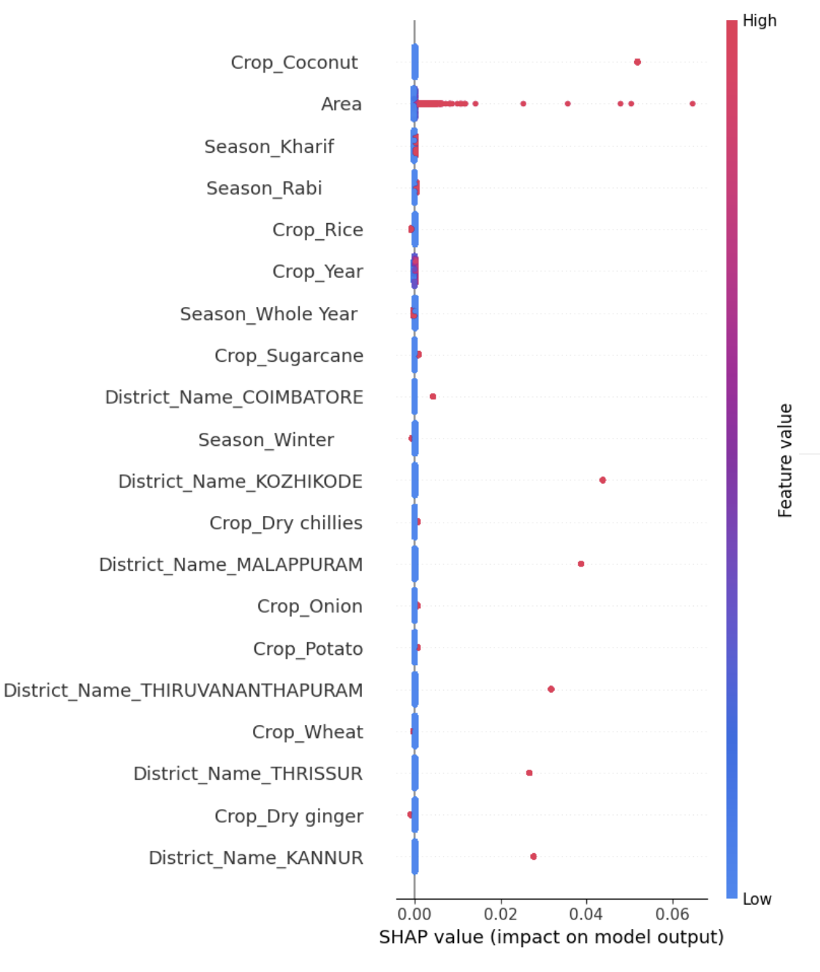
\includegraphics[width=0.75\textwidth]{summary.png}
    \caption{SHAP Summary Plot showing global feature importance}
    \label{fig:shap-summary}
\end{figure}

\subsection{SHAP Force Plot}

\begin{figure}[h!]
    \centering
    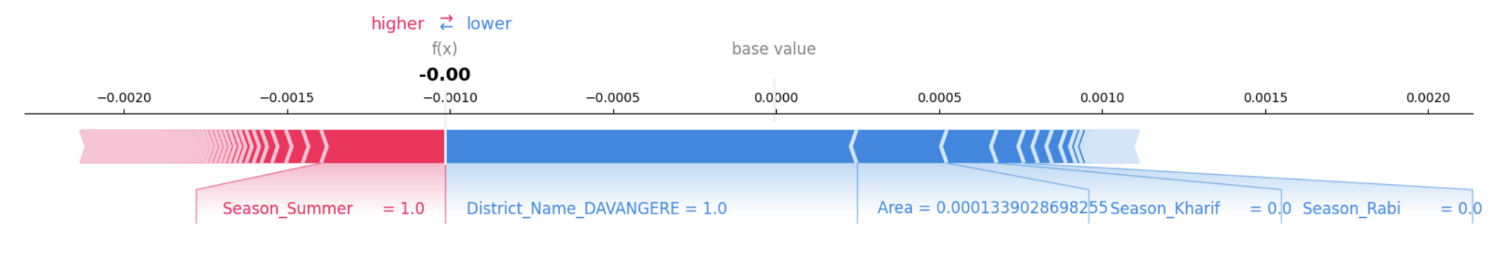
\includegraphics[width=1.0\textwidth]{force.png}
    \caption{SHAP Force Plot showing how features push prediction relative to the baseline}
    \label{fig:shap-force}
\end{figure}

\subsection{SHAP Decision Plot}

\begin{figure}[h!]
    \centering
    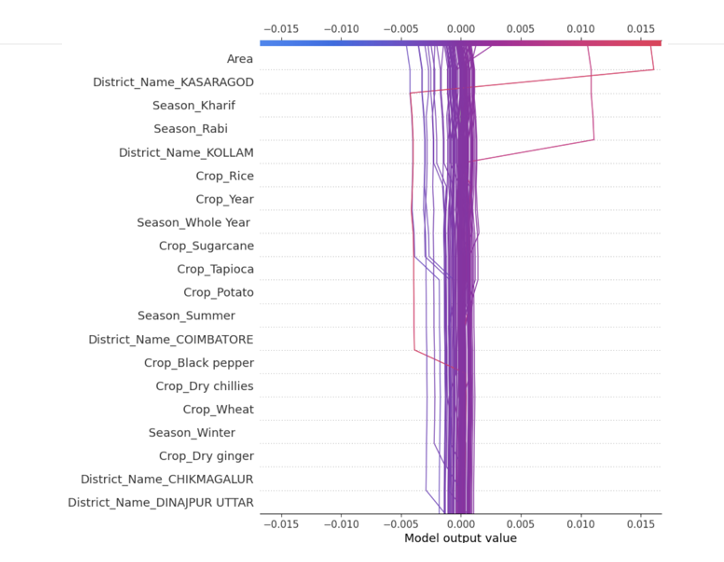
\includegraphics[width=0.8\textwidth]{decision.png}
    \caption{SHAP Decision Plot showing cumulative feature impact across multiple instances}
    \label{fig:shap-decision}
\end{figure}

\subsection{SHAP Waterfall Plot}

\begin{figure}[h!]
    \centering
    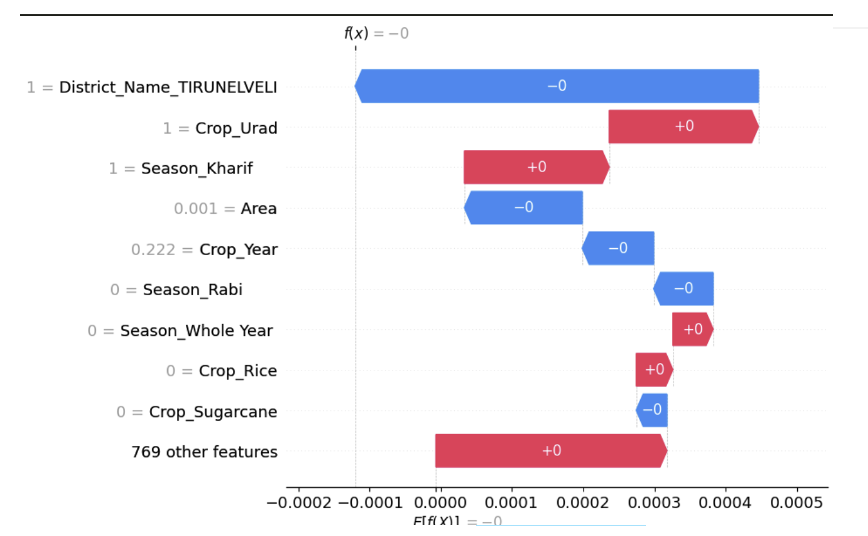
\includegraphics[width=0.7\textwidth]{waterfall.png}
    \caption{SHAP Waterfall Plot visualizing contribution of features to a single prediction}
    \label{fig:shap-waterfall}
\end{figure}

\section{Interpretation of Results}

Key takeaways from SHAP analysis include:
\begin{itemize}
    \item \textbf{Global Insights:} \texttt{Area}, \texttt{Crop Type}, and \texttt{Season} are the most impactful features across the dataset.
    \item \textbf{Local Insights:} District-specific crops (e.g., \texttt{Urad} in \texttt{TIRUNELVELI}) have strong positive influence in those regions.
    \item \textbf{Actionable Interpretation:} Farmers in specific regions can receive model-driven recommendations backed by interpretable plots.
\end{itemize}

\section{Comparison with Traditional Models}

Traditional models like Decision Tree and XGBoost, though useful, did not offer the same level of performance or interpretability as Random Forest + SHAP.

\begin{itemize}
    \item RF + SHAP achieved the lowest MAE and RMSE.
    \item It also produced explainable visualizations aiding real-world decision-making.
\end{itemize}

\section{Summary}

This chapter presented a detailed analysis of model performance and interpretability. The Random Forest model achieved the best accuracy and, when combined with SHAP, provided a transparent and robust yield prediction pipeline. The next chapter concludes the project and outlines future directions for research and deployment.

\newpage

% ----------------- Conclusion and future work -----------------


\chapter{Conclusion and Future Work}

\section{Conclusion}

In this project, we explored the integration of Explainable Artificial Intelligence (XAI) into crop yield prediction systems using SHAP (SHapley Additive exPlanations). The primary objective was to develop a pipeline that not only delivers accurate yield forecasts but also provides transparent explanations for the predictions. This is particularly crucial in the context of agriculture, where trust, interpretability, and decision support are vital for widespread adoption of AI-based solutions.

The project successfully demonstrated the applicability of SHAP in enhancing the interpretability of machine learning models used for yield prediction. Among the models evaluated — Decision Tree, XGBoost, and Random Forest — the Random Forest model provided the best performance with an accuracy of 98.96\%, a Mean Absolute Error (MAE) of 1.97, and a Root Mean Square Error (RMSE) of 2.45.

Using SHAP, we were able to break down individual predictions and attribute them to specific features. Visual tools such as summary plots, force plots, waterfall plots, and decision plots offered rich interpretability, making the prediction process understandable for non-technical stakeholders such as farmers and policymakers.

Key contributions of this work include:
\begin{itemize}
    \item Construction of a robust and interpretable machine learning pipeline using real-world Indian agricultural data.
    \item Comparative performance analysis of multiple models based on accuracy and explainability.
    \item Integration of SHAP to produce both global and local explanations for yield predictions.
    \item Development of meaningful visualizations that aid in decision-making and policy formulation.
\end{itemize}

The explainability framework proved useful in identifying critical factors such as \texttt{Area}, \texttt{Crop Type}, and \texttt{Season} that significantly influence yield predictions. These insights not only enhance transparency but also support targeted interventions for increasing productivity.

\section{Implications of Findings}

The integration of SHAP has notable implications:

\begin{itemize}
    \item \textbf{For Farmers:} The model provides interpretable feedback on how inputs like area and crop type influence predicted yields, guiding planting decisions.
    \item \textbf{For Policymakers:} Region-wise interpretability helps in identifying areas requiring support or optimization.
    \item \textbf{For Researchers:} Demonstrates a replicable framework for combining model performance with interpretability.
\end{itemize}

Thus, this project bridges the gap between AI model performance and real-world usability in the agricultural sector.

\section{Limitations}

While the results are promising, a few limitations remain:
\begin{itemize}
    \item The model is trained on static datasets, which may not capture dynamic environmental or policy changes.
    \item Interpretability is dependent on the SHAP approximation, which, while robust, may not fully represent causal relationships.
    \item The current implementation focuses on district-level data and may require customization for village-level or farmer-specific deployment.
\end{itemize}

\section{Future Work}

This project opens multiple avenues for future research and development:

\begin{itemize}
    \item \textbf{Integration with Real-Time Data:} Incorporating live weather, soil, and satellite data can make the prediction system dynamic and adaptive.
    \item \textbf{Geo-Spatial Visualization:} Developing an interactive map interface to visualize SHAP values at district or state level could improve accessibility and policy support.
    \item \textbf{Farmer-Centric Applications:} A mobile application can be built to allow farmers to enter their data and receive yield forecasts along with SHAP-based explanations in local languages.
    \item \textbf{Extending to Other Crops and Regions:} The current model can be generalized to include additional crops, soil types, and agro-climatic zones.
    \item \textbf{Causal Explainability:} Future models could explore causal inference techniques to complement SHAP values with cause-effect relationships.
    \item \textbf{Model Compression and Deployment:} For practical use in rural settings, lightweight versions of the model can be developed for edge devices with limited computing power.
\end{itemize}

\section{Final Remarks}

This study highlights the growing relevance of explainability in real-world AI applications. By combining predictive accuracy with human interpretability, the proposed system not only supports better agricultural planning but also fosters trust in AI among its users. As agriculture continues to embrace digital transformation, such explainable frameworks are expected to play a foundational role in the future of smart farming.

\newpage

% ----------------- References -----------------

\chapter*{References}
\addcontentsline{toc}{chapter}{References}

\begin{itemize}
    \item A. Chlingaryan, S. Sukkarieh, and B. Whelan, ``Machine learning approaches for crop yield prediction and nitrogen status estimation in precision agriculture: A review,'' \emph{Computers and Electronics in Agriculture}, vol. 151, pp. 61–69, 2018.
    \item J. H. Jeong, J. H. Resop, N. E. Mueller, T. K. Fleisher, D. M. Kim, and A. P. M. Linquist, ``Random Forests for agricultural crop yield predictions,'' \emph{Agricultural and Forest Meteorology}, vol. 216, pp. 60–73, 2016.
    \item B. Liu, W. Jin, and J. Yang, ``An ensemble learning approach for maize yield prediction using remote sensing data,'' \emph{Remote Sensing}, vol. 12, no. 20, pp. 1–16, 2020.
    \item J. You, X. Li, M. Low, D. Lobell, and S. Ermon, ``Deep Gaussian Process for Crop Yield Prediction Based on Remote Sensing Data,'' in \emph{Proc. 31st AAAI Conf. on Artificial Intelligence (AAAI)}, San Francisco, CA, 2017.
    \item S. Khaki and L. Wang, ``Crop Yield Prediction Using Deep Neural Networks,'' \emph{Frontiers in Plant Science}, vol. 10, pp. 621, 2019.
    \item A. Kamilaris and F. X. Prenafeta-Boldú, ``Deep learning in agriculture: A survey,'' \emph{Computers and Electronics in Agriculture}, vol. 147, pp. 70–90, 2018.
    \item A. Barredo Arrieta, N. Díaz-Rodríguez, J. Del Ser, A. Bennetot, S. Tabik, A. Barbado, et al., ``Explainable Artificial Intelligence (XAI): Concepts, taxonomies, opportunities and challenges toward responsible AI,'' \emph{Information Fusion}, vol. 58, pp. 82–115, 2020.
    \item Y. Wang, X. Zhang, and R. Wang, ``Application of SHAP Values for the Interpretation of Disease Risk Prediction Models in Agriculture,'' \emph{IEEE Access}, vol. 9, pp. 15123–15133, 2021.
    \item S. Ghosal, A. Blystone, and A. Singh, ``Explainable AI Models for Disease Detection in Agriculture,'' in \emph{Proc. IEEE Conf. on Computer Vision and Pattern Recognition (CVPR) Workshops}, 2020.
    \item S. M. Lundberg and S.-I. Lee, ``A Unified Approach to Interpreting Model Predictions,'' in \emph{Proc. 31st Advances in Neural Information Processing Systems (NeurIPS)}, pp. 4765–4774, 2017.
\end{itemize}

\newpage


\end{document}
